\documentclass[sn-mathphys-num]{sn-jnl}
%% The project bundle includes a lightweight sn-jnl.cls compatibility shim so
%% this manuscript can compile in a clean Overleaf project. For a journal
%% submission, replace the shim with the official Springer Nature class files.

\usepackage{booktabs}
\usepackage{graphicx}
\usepackage{amsmath,amssymb}
\usepackage{array,multirow}
\usepackage{siunitx}
\usepackage{placeins}
\usepackage{enumitem}
\usepackage{xcolor}
\usepackage[colorlinks=true,linkcolor=black,citecolor=black,urlcolor=blue!55!black]{hyperref}
\usepackage[capitalise,noabbrev]{cleveref}
\usepackage{orcidlink}

\graphicspath{{figures/}{../figures/}}
\sisetup{detect-all,group-minimum-digits=4}

\definecolor{pmred}{HTML}{E4572E}
\definecolor{tmblue}{HTML}{2E86AB}
\definecolor{xgbgreen}{HTML}{2E9E5B}
\definecolor{panel}{HTML}{F4F6F8}
\definecolor{ink}{HTML}{23313F}

\newcommand{\PM}{\mathrm{PM}_{2.5}}
\newcommand{\TM}{\textsc{TimeMixer}}
\newcommand{\XGB}{\textsc{XGBoost}}
\newcommand{\HYB}{\textsc{TM-XGB}}
\newcommand{\Exp}{\mathbb{E}}
\newcommand{\Real}{\mathbb{R}}
\newcommand{\Horizons}{\{1,6,12,24,48\}}
\newcommand{\given}{\,\vert\,}

\title{A Hybrid TimeMixer-XGBoost Framework for Multi-Horizon PM2.5 Forecasting Using Historical PM2.5 Time-Series Data}

\author[1]{\fnm{Thu} \sur{Le}
\textnormal{ (0009-0008-3480-8311)}}
\email{thulvm@fpt.edu.vn}

\author[1]{\fnm{Nhi} \sur{Tran}
\textnormal{ (0009-0001-1047-5080)}}
\email{nhikl12006@gmail.com}

\author[1]{\fnm{Han} \sur{Dong}
\textnormal{ (0009-0002-2532-8099)}}
\email{donghan010106@gmail.com}

\author[1]{\fnm{Ngan} \sur{Pham}
\textnormal{ (0009-0001-1089-2626)}}
\email{tunganphamhoang@gmail.com}

\affil{
  \orgdiv{Faculty of Information Technology},
  \orgname{FPT University},
  \orgaddress{
    \city{Ho Chi Minh City},
    \country{Vietnam}
  }
}

\affil[]{
  \textbf{Emails:}
  \texttt{thulvm@fpt.edu.vn};
  \texttt{nhikl12006@gmail.com};
  \texttt{donghan010106@gmail.com};
  \texttt{tunganphamhoang@gmail.com}
}

\abstract{Accurate multi-horizon PM2.5 forecasting is difficult because hourly
monitoring records combine persistence, periodicity, abrupt episodes,
missing observations, site heterogeneity, and measurement-regime changes.
This study evaluates a calibration-gated TimeMixer-XGBoost framework at five
UK-Air stations and horizons of 1, 6, 12, 24, and 48 hours. The residual stage
removes calibration-period median bias, fits horizon-specific XGBoost models
with pseudo-Huber loss and bounded corrections, selects a correction scale on
a later held-out calibration subset, and applies rolling calibration using
only errors observable at each forecast origin. The benchmark includes
persistence, seasonal-naive, direct XGBoost, DLinear, LSTM, TimeMixer,
ungated robust correction, gated static correction, and gated rolling
correction. Neural experiments use seeds 0-4 and a 30-epoch maximum under
separate training, early-stopping, residual-fit, gate-selection, and
locked-test eras. The confirmatory experiment completed five stations, five seeds, and a 30-epoch maximum. The hybrid won 0/25 comparisons against the strongest matched non-hybrid comparator, giving a 23.33\% MAE gap, but improved compact TimeMixer and prevented severe ungated over-correction. LSTM (MAE 3.271) and DLinear (3.282) were practically tied; DLinear led pooled RMSE and sMAPE. Common-history sensitivity changed hybrid MAE by only \( +0.012 \), so the result is a leakage-controlled negative finding, not a state-of-the-art claim.
}

\keywords{PM2.5; TimeMixer; XGBoost; multi-horizon forecasting; air quality; residual learning; time-series forecasting; reproducibility}

\begin{document}
\maketitle
\section{Introduction}
\label{sec:intro}

An air-quality monitor reports what was observed; a forecasting system must estimate what will occur before the next exposure period. The distinction matters because the value of an alert depends on lead time as well as accuracy. The World Health Organization's 2021 guidelines summarize extensive evidence linking particulate exposure with respiratory and cardiovascular harm~\cite{who2021aqg}. Operational forecasts must therefore remain reliable across several lead times, behave sensibly during elevated concentrations, and fail visibly when the monitoring record is incomplete.

Roadside PM2.5 is a difficult target because a single hourly series mixes persistence, traffic-related variation, daily and weekly cycles, seasonal structure, transported pollution, abrupt local events, and measurement noise. Missingness further complicates evaluation: a short bounded gap may be reconstructed conservatively, whereas a multi-week outage cannot be filled without fabricating a long synthetic trajectory. Instrument replacement can also shift the observation process and create a predictive regime change that is confounded with calendar time.

Different model families address complementary parts of this structure. LSTM networks model sequential dependence through gated recurrent states~\cite{hochreiter1997lstm}; XGBoost captures nonlinear interactions among lagged, rolling, and calendar predictors~\cite{chen2016xgboost}; and TimeMixer represents multiple temporal scales through downsampling, decomposition, and cross-scale mixing~\cite{wang2024timemixer}. This motivates a division of labor: a multiscale neural model can produce the main trajectory forecast, while a boosted tree model attempts to learn the structured residual error that remains.

We test that hypothesis in a deliberately constrained historical-PM2.5 setting. One week (168 hours) of origin-available sequence information is used to predict PM2.5 directly at $t+1$, $t+6$, $t+12$, $t+24$, and $t+48$ hours. No forecast-time weather, traffic, emissions, satellite, or neighboring-station inputs are required. The restriction isolates the autoregressive and calendar signal; it is not a claim that these physical drivers are unimportant.

The architecture contains a frozen representation stage and a guarded
residual stage. TimeMixer produces a five-horizon forecast vector and
multiscale embedding. The residual stage removes calibration-period median
bias, fits horizon-specific XGBoost models with pseudo-Huber loss and bounded
corrections, uses a later calibration subset to suppress harmful corrections,
and then applies rolling calibration using only errors whose targets are
already observable at the forecast origin.

The revised study asks whether the robust rolling hybrid improves over the strongest matched comparator, whether gains replicate across station types and horizons, and which residual safeguard contributes to any improvement. The evaluation adds DLinear, multiple stations, five random seeds, and a 30-epoch maximum. No state-of-the-art claim is permitted unless the completed matched benchmark and paired uncertainty support it.

\section{Related Work}
\label{sec:related}

Classical PM2.5 forecasting methods remain useful because the series is strongly autocorrelated and seasonal, but fixed linear structure can be restrictive for abrupt nonlinear dynamics. LSTM remains a standard sequence comparator~\cite{hochreiter1997lstm}; decomposition-based LSTM ensembles also illustrate the value of separating temporal modes before nonlinear learning~\cite{bai2019ensemble}. Relative performance can change with input design and lead time, which motivates horizon-specific reporting~\cite{beijing2021forecast}.

Modern long-sequence forecasting emphasizes local patches, frequency structure, and multiresolution representations. PatchTST tokenizes subsequences~\cite{nie2023patchtst}, while TimeMixer downsamples, decomposes, and mixes information across temporal scales~\cite{wang2024timemixer}. XGBoost is complementary because it can model nonlinear interactions among lag, rolling, calendar, and regime features~\cite{chen2016xgboost}; in a hybrid design, it can target the conditional residual of a frozen sequence model rather than relearning the full trajectory.

Evaluation must respect chronology and serial dependence. The experiment therefore uses successive time intervals, common-origin comparisons, MAE as the primary endpoint~\cite{willmott2005mae}, paired Diebold-Mariano tests~\cite{diebold1995accuracy}, and autocorrelation-aware variance estimation motivated by HAC inference~\cite{newey1987hac}. Reproducibility is treated as part of the method: reported results are generated from saved experiment outputs rather than manually typed placeholder values.

\section{From Historical PM2.5 Time Series to Multi-Horizon Residual Correction}
\label{sec:framework}

We develop the method in one arc: the audited station record, the conservative cleaning operator, leakage-safe forecast-origin construction, the multiscale base forecaster, and the residual correction stage. The key methodological principle is separation: raw evidence is separated from modeling values, short-gap interpolation from long-gap preservation, representation learning from residual calibration, and model selection from locked testing.

\subsection{Setup}
\label{sec:site}

The confirmatory dataset contains five UK-Air stations selected to represent
different monitoring environments: London Marylebone Road (MY1, urban
traffic), Birmingham A4540 (BIR\_A4540, urban traffic), London Honor Oak Park
(HP1, urban background), Chilbolton (CHB, rural background), and London North
Kensington (KC1, urban background). Each station is processed independently
with the same schema, cleaning rules, forecast horizons, chronological
boundaries, seeds, and evaluation metrics. Dataset paths and site types are
fixed in \texttt{data/stations.csv}.

UK-Air exports separate date and hour-ending time fields. During ingestion,
the pipeline preserves source filename, source row identity, raw timestamp
text, raw concentration text, and status metadata. A source time of 24:00 is
normalized to 00:00 of the following day. The target is hourly PM2.5 mass
concentration in \si{\micro\gram\per\cubic\meter}.

\begin{table*}[tbp]
\centering
\caption{Station-specific data limitations identified before model fitting.}
\label{tab:station-quality}
\small
\begin{tabular}{llll}
\toprule
Station & Type & Available-history issue & Pre-specified treatment \\
\midrule
MY1 & Urban traffic & 2020 coverage 77.81\%; 69-day gap & Preserve long gap; reject affected windows \\
BIR\_A4540 & Urban traffic & Record begins in 2021 & Report shorter training history \\
HP1 & Urban background & No observations in 2016-2018 & Treat as unavailable, not imputed \\
CHB & Rural background & 2024 coverage 73.44\%; 561 negatives & Mask negatives; preserve unresolved gaps \\
KC1 & Urban background & Instrument-regime transition & Retain instrument type as context \\
\bottomrule
\end{tabular}
\end{table*}

These differences imply unequal amounts of usable training history in the
primary analysis. The primary design uses every station's legitimately
available history because this reflects the operational archive. A
pre-specified common-history sensitivity analysis instead restricts all
training inputs and targets to 1 January 2021 through 31 December 2022, while
leaving the 2023 validation, January-June 2024 calibration, and locked test
period unchanged.

\subsection{Auditable cleaning and the missingness operator}
\label{sec:cleaning}

The raw file is immutable. Cleaning creates three concentration concepts. The \emph{raw} field preserves source evidence. The \emph{observed} field contains numeric, non-negative measurements before imputation. The \emph{clean} field adds only approved short-gap interpolation. Each row carries flags for timestamp validity, missing or non-numeric source values, negative values, duplicate timestamps, inserted hourly-grid rows, interpolation, and preserved long gaps.

The audit identifies 8,087 missing or non-numeric readings before negative handling and 238 additional numeric values below zero. Negative values are masked only in the modeling field; the raw value remains auditable. Duplicate timestamps, if present, are resolved deterministically after sorting by timestamp and source row. The series is then reindexed to an exact one-hour grid so that a missing row and a present row containing ``No data'' have the same modeling implication while remaining distinguishable in the audit.

Instrument information is parsed from the status field and encoded as TEOM FDMS $=0$ and BAM $=1$. Instrument metadata may be propagated across grid-only rows because this describes the observation regime, whereas concentration values are not propagated. Status metadata identify a TEOM FDMS-to-BAM transition at 12:00 UTC on 22 December 2021.

For each contiguous invalid run, the cleaning stage records start time, end time, duration, class, and the number of inserted rows. Linear interpolation is allowed only when a run is internal, bounded by observed values on both sides, and no longer than three hours. Runs of 4-24 hours, 25-168 hours, and more than seven days remain missing. The maximum invalid run is 1,656 hours, exactly 69 days, and is therefore preserved. Any model sequence or requested target containing unresolved missingness is rejected and counted.

\begin{table}[tbp]
\centering
\caption{Verified quality profile of the supplied London Marylebone Road record.}
\label{tab:dataaudit}
\small
\begin{tabular}{lr}
\toprule
Audit item & Value \\
\midrule
Raw hourly rows & \num{87672} \\
Missing/non-numeric readings & \num{8087} \\
Negative numeric measurements & \num{238} \\
Longest invalid run & \num{1656} h (69 d) \\
2020 valid coverage after negative exclusion & 77.81\% \\
Instrument transition & 22 Dec 2021, 12:00 UTC \\
Primary short-gap interpolation limit & 3 h \\
\bottomrule
\end{tabular}
\end{table}

\subsection{Origin-safe predictors and a leakage invariant}
\label{sec:originsafe}

Calendar predictors contain hour, day of week, month, day of year, weekend status, and sine/cosine encodings for hour, weekday, and annual position. The direct XGBoost baseline uses PM2.5 lags at 1, 2, 3, 6, 12, 24, 48, 72, and 168 hours; rolling mean, standard deviation, minimum, maximum, and median over 3, 6, 12, 24, 48, and 168 hours; one- and 24-hour differences; a 24-hour ratio; cyclic calendar variables; and instrument type.

Every rolling statistic is computed from the series after a one-hour shift. Thus, a rolling feature attached to origin $t$ contains values no later than $t-1$. The current PM2.5 value $y_t$ remains available as the last element of the 168-hour sequence and to persistence. This convention corresponds to issuing a forecast after the latest observation has arrived.

\begin{proposition}[Origin-safety of the constructed predictors]
\label{prop:leakage}
For a forecast origin $t$, every sequence, lag, rolling, calendar, instrument, and missingness predictor constructed by the pipeline is measurable from timestamps no later than $t$. Every target is strictly later than $t$ and is constrained to remain inside its assigned chronological partition.
\end{proposition}

\begin{proof}
The sequence terminates at the origin; lag features are explicit backward shifts; rolling summaries are computed from a series shifted by one hour; calendar, instrument, and missingness context are read from the origin or its past; and the window constructor accepts targets only at positive configured horizons. A partition-specific target-end constraint rejects any origin whose furthest requested target would cross the partition boundary. Therefore, no target-side value enters a predictor and no target crosses into a later experimental era.
\end{proof}

This invariant is important because multi-horizon sequence windows overlap heavily. A random split would place nearly identical historical contexts on both sides of a boundary, whereas chronological partitions preserve the information set that would exist at deployment.

\subsection{Forecasting problem}
\label{sec:problem}

Let $y_t$ denote hourly PM2.5 and let
\begin{equation}
\mathbf{x}_{t-L+1:t}\in\Real^{L\times p}
\end{equation}
be the origin-available sequence with $L=168$ hours and $p=9$ channels. The sequence channels are cleaned PM2.5, a missingness mask, instrument type, and cyclic hour, weekday, and annual encodings. For horizon set $\mathcal H=\Horizons$, the direct task is
\begin{equation}
\hat{\mathbf y}_t=
\left(\hat y_{t+1},\hat y_{t+6},\hat y_{t+12},\hat y_{t+24},\hat y_{t+48}\right).
\end{equation}
Predictions are generated simultaneously and are not recursively fed back. Direct prediction avoids recursive error accumulation and permits one residual correction function per horizon.

\begin{table}[tbp]
\centering
\caption{Core notation.}
\label{tab:notation}
\small
\begin{tabular}{ll}
\toprule
Symbol & Meaning \\
\midrule
$y_t$ & observed hourly PM2.5 at time $t$ \\
$L$ & input history length, fixed at 168 h \\
$\mathcal H$ & direct horizon set $\Horizons$ h \\
$\mathbf{x}_{t-L+1:t}$ & origin-available multichannel sequence \\
$\hat{\mathbf y}^{TM}_t$ & TimeMixer base forecast vector \\
$\mathbf e_t$ & flattened multiscale TimeMixer embedding \\
$\mathbf z_t$ & calendar, instrument, and missingness context \\
$r_{t,h}$ & TimeMixer residual at horizon $h$ \\
$g_h(\cdot)$ & XGBoost residual model for horizon $h$ \\
$\gamma_h$ & held-out calibration correction gate for horizon $h$ \\
\bottomrule
\end{tabular}
\end{table}

\subsection{Compact TimeMixer base forecaster}
\label{sec:timemixer}

The implementation is a compact research adaptation of the core multiscale ideas in TimeMixer rather than a claim of line-for-line equivalence to the full benchmark implementation~\cite{wang2024timemixer}. For scales $s\in\{1,2,4,8\}$, the input sequence is average-pooled with stride $s$ to produce $\mathbf{x}^{(s)}$. A centered moving average of kernel 25 estimates a smooth component $\mathbf{t}^{(s)}$, while
\begin{equation}
\mathbf{q}^{(s)}=\mathbf{x}^{(s)}-\mathbf{t}^{(s)}
\end{equation}
acts as a residual seasonal component. Separate two-layer MLP encoders map $\mathbf{q}^{(s)}$ and $\mathbf{t}^{(s)}$ to 64-dimensional summaries. Their concatenation is fused into a scale representation $\mathbf e^{(s)}$.

Two mixer blocks alternate residual MLP transformations across the scale axis and the hidden-feature axis with layer normalization. A linear prediction head at each scale produces five horizon forecasts. Learned softmax weights combine them:
\begin{equation}
\hat{\mathbf y}^{TM}_t=\sum_s \alpha_s f_s\left(\mathbf e_t^{(s)}\right),
\qquad
\alpha_s=\frac{\exp(a_s)}{\sum_j\exp(a_j)}.
\end{equation}
The mixed representations are flattened into
\begin{equation}
\mathbf e_t=
\left[\mathbf e_t^{(1)};\mathbf e_t^{(2)};\mathbf e_t^{(4)};\mathbf e_t^{(8)}\right]
\end{equation}
for residual calibration. Huber loss, AdamW optimization, gradient clipping, and early stopping are used. Input and target standardizers are fitted on training windows only.

\subsection{Horizon-specific residual XGBoost}
\label{sec:residual}

The residual-calibration interval is divided chronologically into an earlier
residual-fit subset $\mathcal C_f$ (70\%) and a later gate-selection subset
$\mathcal C_g$ (30\%). For each horizon $h$, the residual is first centred by
the median $b_h$ estimated only on $\mathcal C_f$, after which a separate
robust booster learns the remaining error:
\begin{align}
r_{t,h}&=y_{t+h}-\hat y^{TM}_{t,h},\qquad
b_h=\operatorname{median}_{t\in\mathcal C_f}(r_{t,h}),\\
\hat u_{t,h}&=g_h\left(\hat{\mathbf y}^{TM}_t,\mathbf e_t,\mathbf z_t\right),\\
\hat c_{t,h}&=b_h+\operatorname{clip}(\hat u_{t,h},q_h^-,q_h^+),\\
\gamma_h&=\arg\min_{\gamma\in\Gamma}
\sum_{t\in\mathcal C_g}
\left|y_{t+h}-(\hat y^{TM}_{t,h}+\gamma\hat c_{t,h})\right|,\\
\hat y^{static}_{t,h}&=\hat y^{TM}_{t,h}+\gamma_h\hat c_{t,h},\\
\hat y^{HYB}_{t,h}&=\hat y^{static}_{t,h}+
\lambda_t\operatorname{median}(\mathcal E_{t,h}).
\end{align}
Here $\Gamma=\{0,0.10,0.25,0.50,0.75,1\}$. The explicit choice
$\gamma_h=0$ falls back to the TimeMixer base when the correction does not
improve held-out calibration MAE. The context vector $\mathbf z_t$ contains
the origin-safe lag and shifted rolling features used by direct XGBoost,
instrument type, cyclic calendar variables, missingness state, gap length,
interpolation status, and measurement-quality flags. The complete base
forecast vector and latent embedding are also supplied to every horizon
model.

Each residual booster uses pseudo-Huber loss, 600 trees, maximum depth 5,
learning rate 0.04, row and feature subsampling of 0.8, minimum child weight
3, and $L_1/L_2$ regularization. Correction bounds $(q_h^-,q_h^+)$ are
estimated on $\mathcal C_f$. The rolling set $\mathcal E_{t,h}$ contains only
errors from the previous 30 days whose target timestamps are no later than
origin $t$; shrinkage $\lambda_t$ prevents unstable updates when few errors
are available. Thus robust fitting, gate selection, and locked testing occupy
strictly ordered intervals.

\IfFileExists{figures/00_framework.png}{
\begin{figure*}[tbp]
\centering

\includegraphics[width=\textwidth]{00_framework.png}
\caption{End-to-end hybrid forecasting framework. Data-quality decisions are completed before sequence construction. TimeMixer produces a direct multi-horizon base forecast and multiscale embedding; XGBoost learns one residual correction per horizon from a later chronological calibration interval. The locked test is evaluated only after both stages are frozen.}
\label{fig:framework}
\end{figure*}}{}

\section{Experimental Setup}
\label{sec:setup}

\paragraph{Chronological partitions.}
The timeline is divided into four consecutive eras. Training through 31 December 2022 fits scalers, neural weights, and direct XGBoost. The year 2023 is reserved for neural early stopping. The interval 1 January-30 June 2024 fits residual XGBoost and pre-specified ablations. The period after 30 June 2024 is locked for final evaluation. Boundary sequences may use earlier history available operationally, but every target must remain inside its own partition.

\begin{table}[tbp]
\centering
\caption{Temporal partitions and permitted use.}
\label{tab:splits}
\small
\begin{tabular}{p{0.22\linewidth}p{0.31\linewidth}p{0.37\linewidth}}
\toprule
Partition & Period & Permitted use \\
\midrule
Training & through 31 Dec 2022 & scalers; neural weights; direct XGBoost \\
Neural validation & 1 Jan-31 Dec 2023 & early stopping only \\
Hybrid calibration & 1 Jan-30 Jun 2024 & residual fit (first 70\%); gate selection (last 30\%) \\
Locked test & after 30 Jun 2024 & final paired evaluation only \\
\bottomrule
\end{tabular}
\end{table}

\paragraph{Comparators and training.}
Persistence, seasonal-naive, direct XGBoost, DLinear~\cite{zeng2023dlinear}, LSTM, and TimeMixer are evaluated as non-hybrid comparators. The static robust residual model and the rolling-calibrated hybrid isolate the effect of each residual safeguard. Neural models use seeds 0-4, batch size 128, AdamW learning rate $10^{-3}$, weight decay $10^{-4}$, gradient clipping at 1.0, patience seven, and a maximum of 30 epochs. All stations use the same pre-specified configuration.

\paragraph{Common-history sensitivity analysis.}
The confirmatory analysis allows each station to use all observations
available before the common training cutoff. Because BIR\_A4540 begins in
2021, this produces unequal training-history lengths. We therefore repeat the
complete five-seed experiment after setting a common training start of
1 January 2021 for every station. Forecast horizons, model hyperparameters,
validation, residual calibration, locked-test timestamps, and eligible-origin
rules remain unchanged. We report the common-minus-available-history change in
MAE and RMSE by station, model, and horizon. Agreement of the model ranking and
hybrid effect across the two analyses supports robustness to training-history
length; disagreement is reported as a limitation rather than resolved by
selecting the more favorable analysis.

\paragraph{Metrics and paired evidence.}
Primary MAE is reported separately by horizon. Secondary metrics are RMSE, sMAPE, $R^2$, and signed bias, evaluated on the common intersection of finite predictions. High-concentration behavior uses the 90th percentile of training PM2.5 as a fixed analytical threshold and reports conditional MAE, recall, and false-alarm rate.

A paired moving-block bootstrap resamples 24-hour blocks of
\begin{equation}
d_{t,h}=|y_{t+h}-\hat y^{HYB}_{t,h}|-|y_{t+h}-\hat y^{TM}_{t,h}|.
\end{equation}
One thousand replicates estimate a percentile 95\% interval for $\bar d_h$; negative values favor the hybrid. A two-sided Diebold-Mariano test~\cite{diebold1995accuracy} uses absolute-error loss with Bartlett-weighted autocovariance up to 24 lags, followed by Holm correction across five horizons. Four same-origin residual variants compare the full hybrid with no embedding, no origin context, and base-forecast-only correction. SHAP summaries are reported by horizon, and all forecast claims are tied to saved locked-test outputs.

\section{Results}
\label{sec:results}

\subsection{The data-quality problem is material, not cosmetic}
\label{sec:results-data}

The first empirical finding is that preprocessing choices materially change
the admissible forecasting sample. At MY1, the record contains 8,087 missing
or non-numeric readings, 238 negative values, and a 1,656-hour maximum invalid
run. Cross-station auditing reveals additional heterogeneity: HP1 contains no
observations in 2016-2018; BIR\_A4540 begins in 2021; CHB has only 73.44\%
coverage in 2024 and contains 561 negative source values; and KC1 contains an
instrument-regime transition. None of these intervals or negative values is
reconstructed through long-range interpolation. Instead, invalid values
remain auditable and forecast windows crossing unresolved gaps are excluded.

\IfFileExists{../figures/01_data_overview.png}{
\begin{figure*}[tbp]
\centering
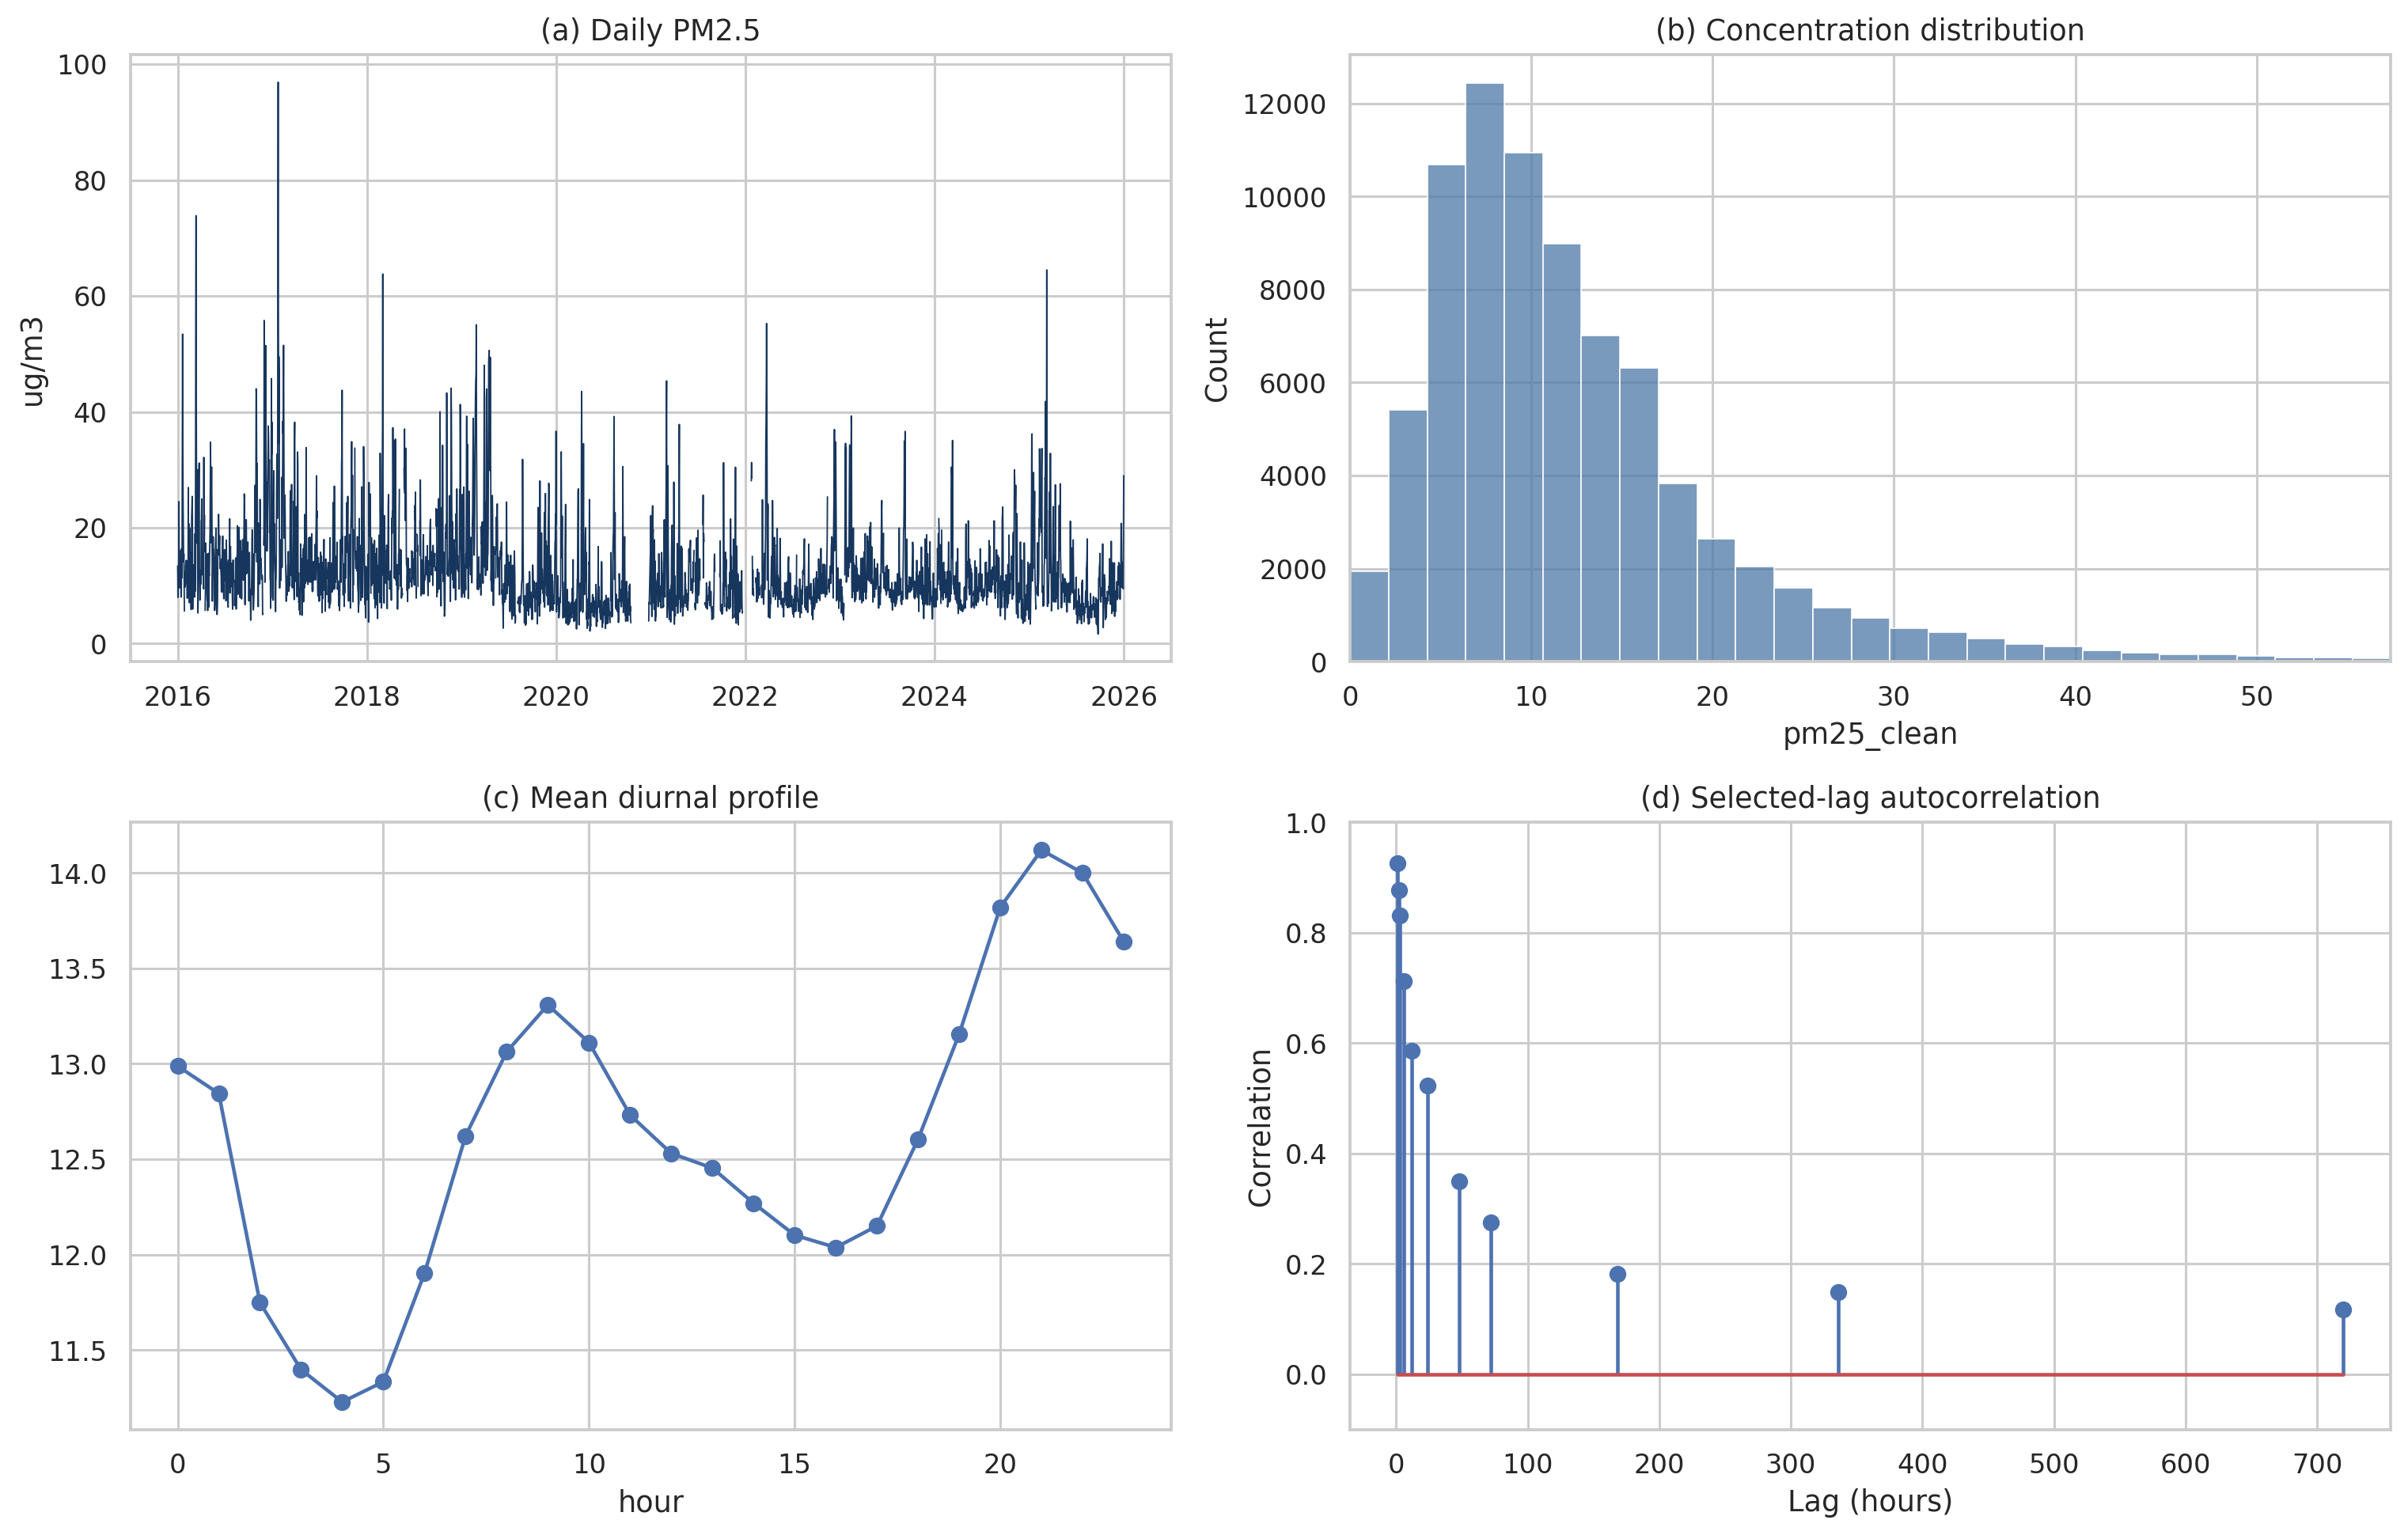
\includegraphics[width=\textwidth]{01_data_overview.png}
\caption{Compact EDA overview: daily PM2.5, concentration distribution, diurnal profile, and selected-lag autocorrelation.}
\label{fig:data-overview}
\end{figure*}}{}

\IfFileExists{../figures/02_data_quality.png}{
\begin{figure*}[tbp]
\centering
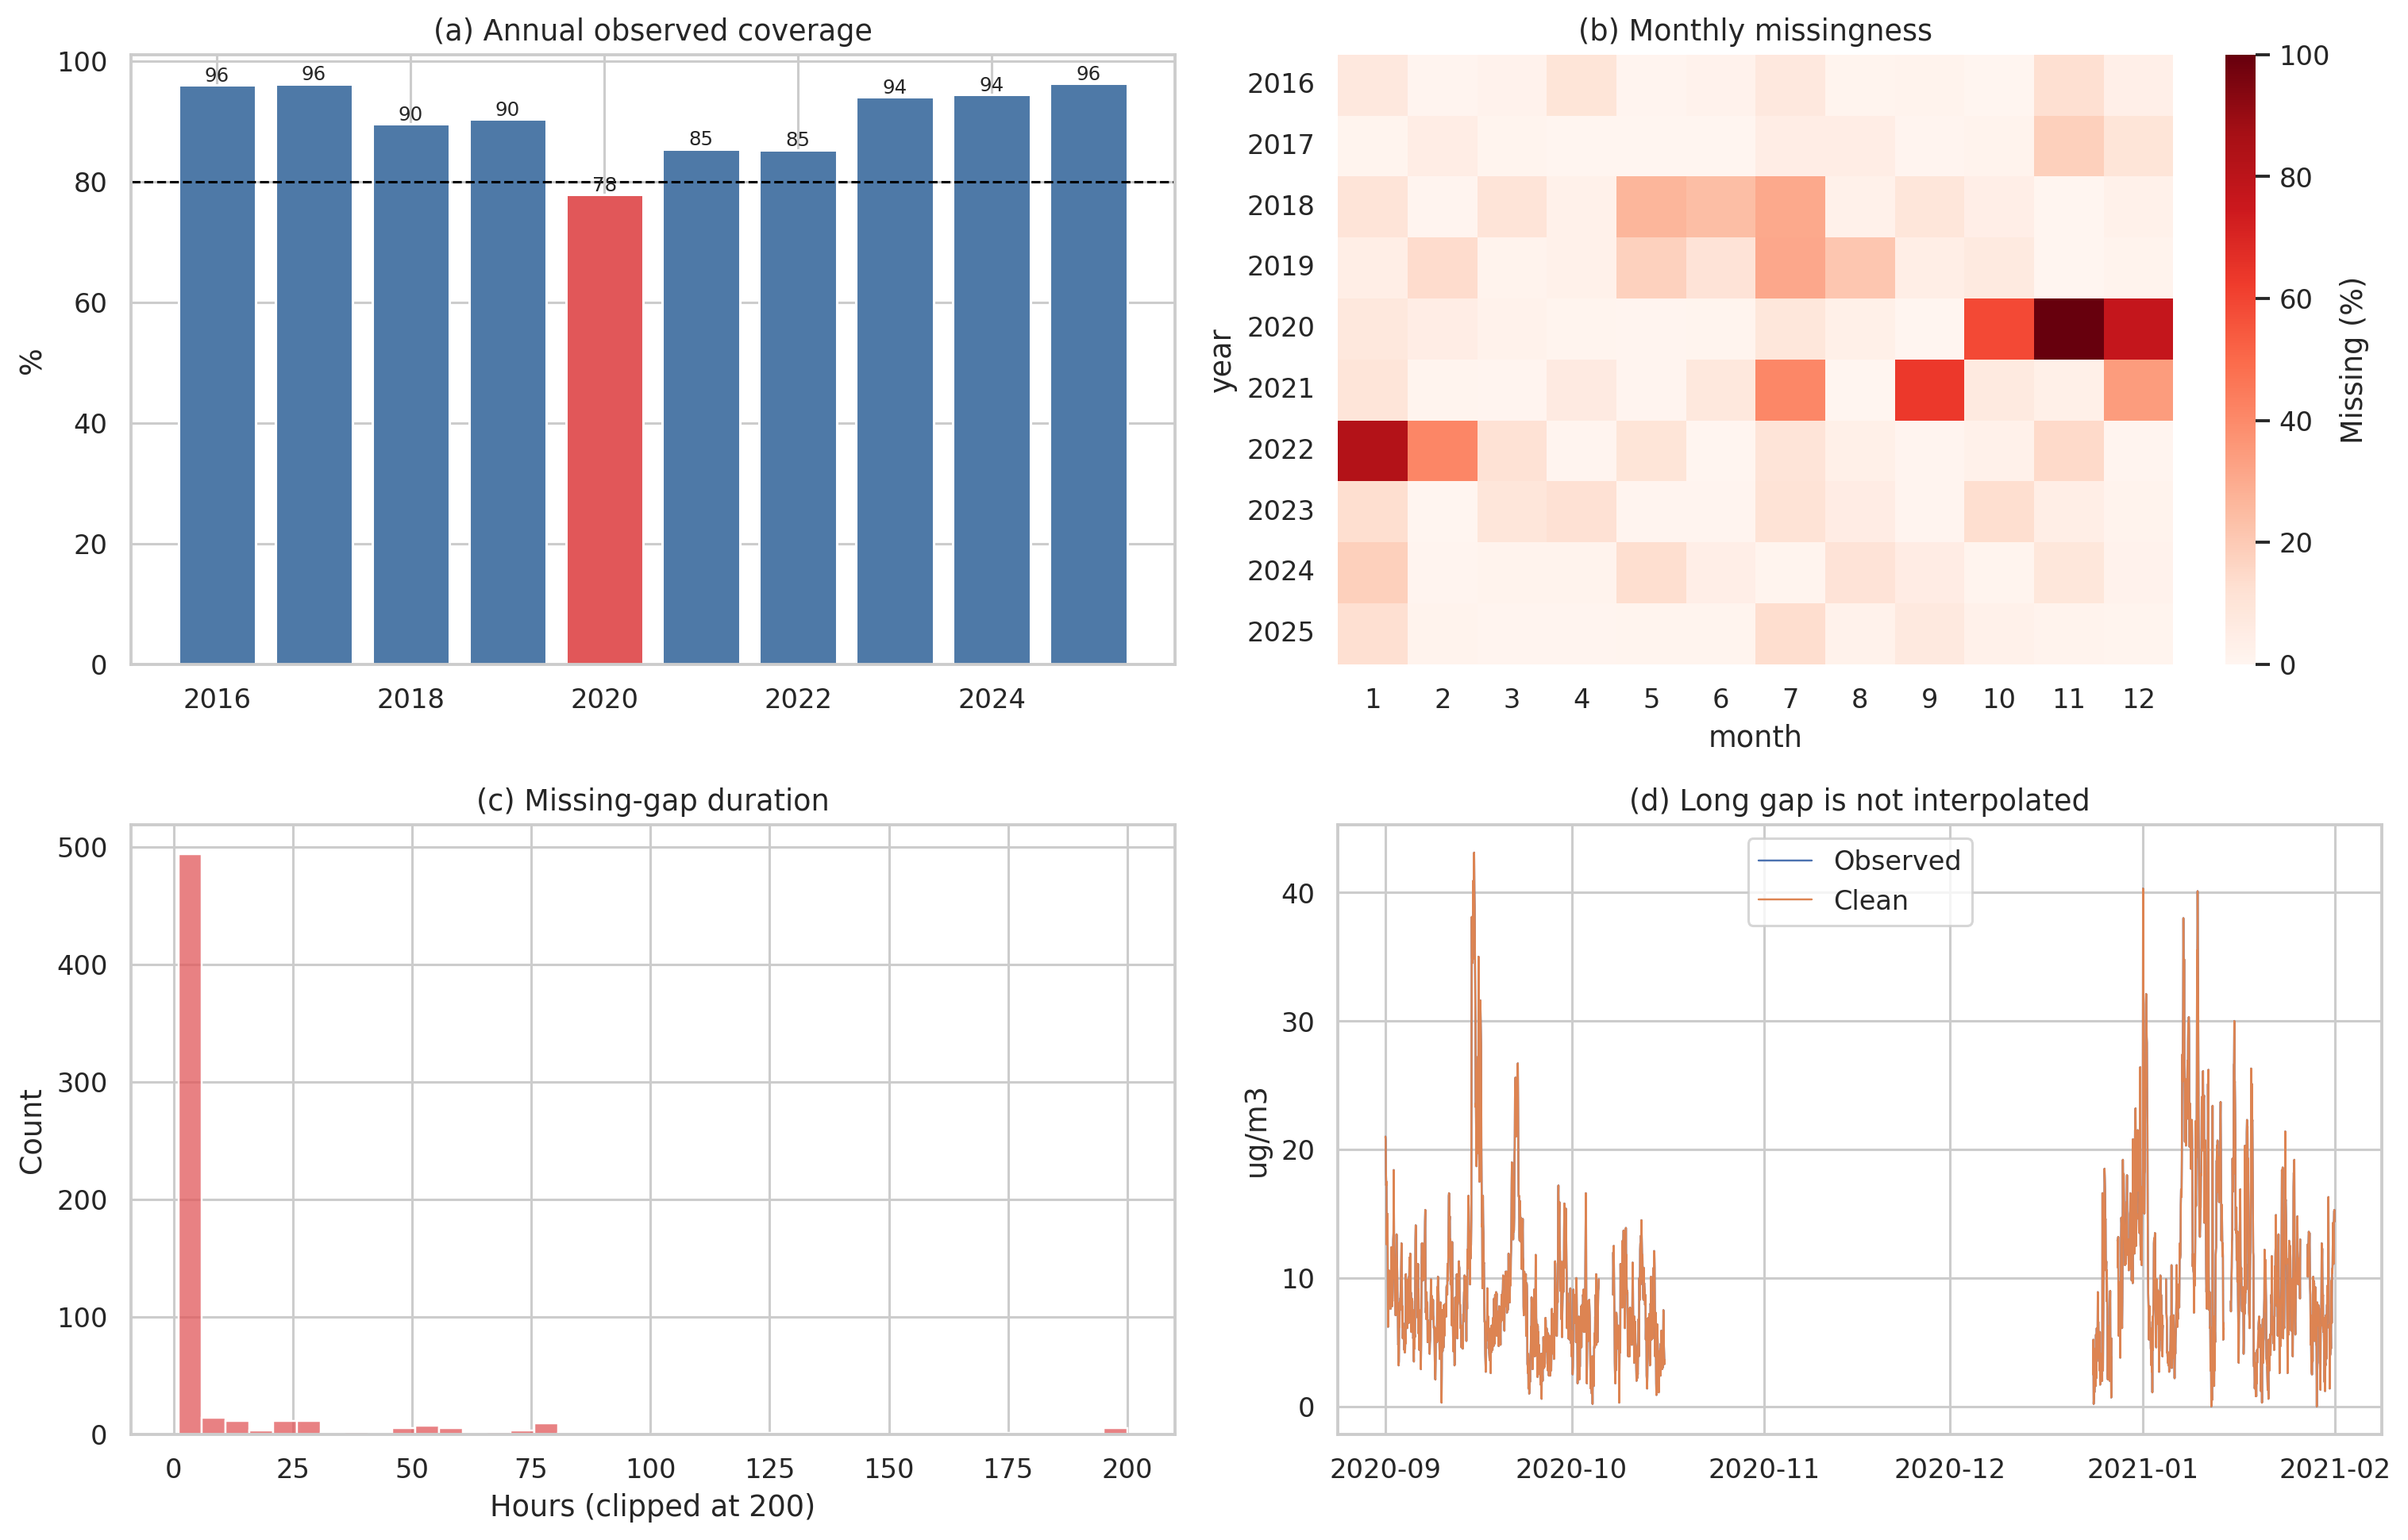
\includegraphics[width=\textwidth]{02_data_quality.png}
\caption{Compact data-quality audit: annual coverage, monthly missingness, gap duration, and the preserved long outage.}
\label{fig:data-quality}
\end{figure*}}{}

The missingness pattern is not independent and identically distributed. Coverage changes across years and clusters by month. Consequently, complete-window evaluation samples the monitoring process as well as the pollution process. This motivates annual coverage reporting, explicit rejected-window counts, and sensitivity analysis over short-gap limits rather than a single opaque imputation pass.

\subsection{The record contains structure at several forecast-relevant scales}
\label{sec:results-eda}

Descriptive profiles show persistent short-lag dependence together with repeating calendar structure. Selected autocorrelations remain informative at daily and weekly lags, supporting both a 168-hour input window and 24/168-hour engineered features. The concentration distribution is right-skewed and contains episodic peaks, so RMSE and high-event metrics complement MAE. The distribution also differs across TEOM FDMS and BAM eras. Because instrument replacement and calendar time move together, this difference cannot be attributed to the instrument alone; instrument type is therefore used only as a predictive regime marker.

The nine single-purpose EDA plots are retained in
\texttt{figures/supplementary/} and are generated by the same plotting code.
\FloatBarrier

\subsection{Locked-test forecast accuracy and statistical evidence}
\label{sec:results-forecast}

\IfFileExists{../figures/03_multistation_effectiveness.png}{
\begin{figure*}[tbp]
\centering
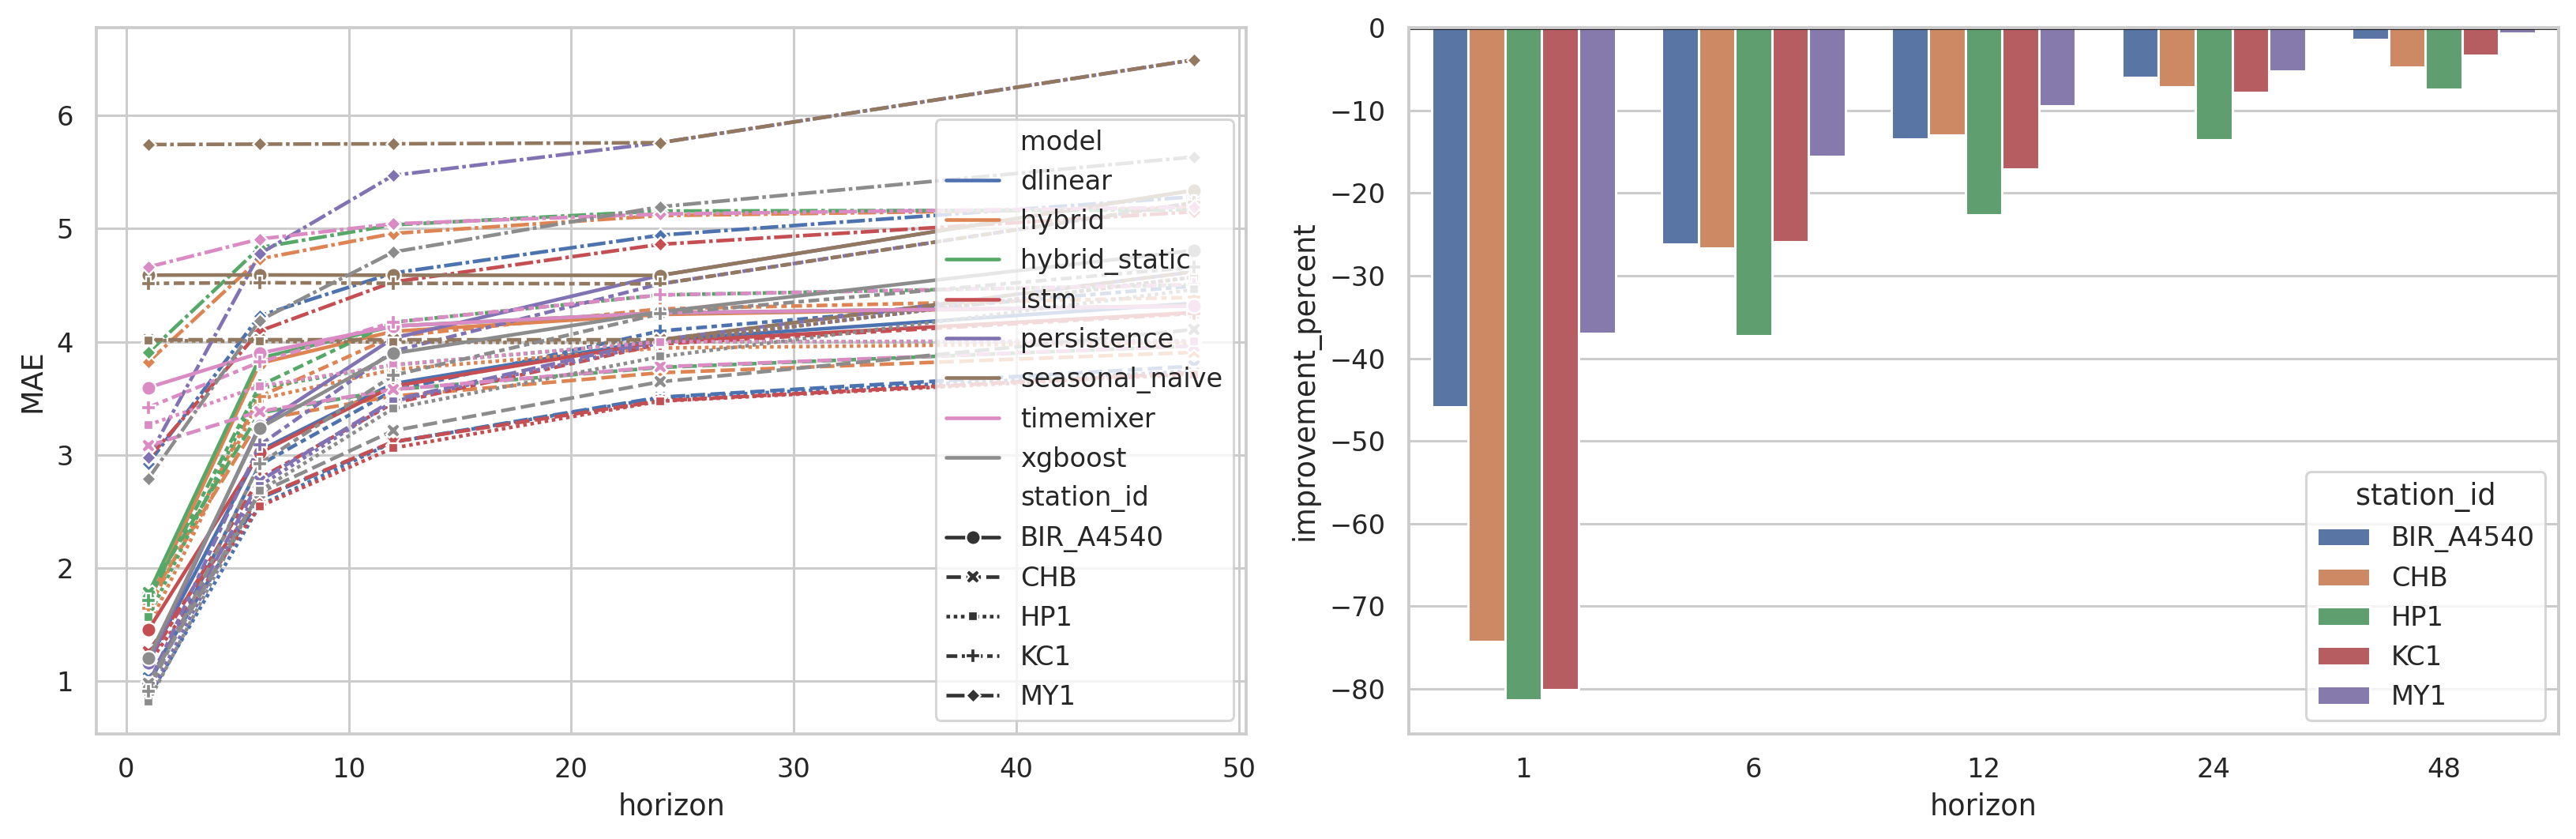
\includegraphics[width=\textwidth]{03_multistation_effectiveness.png}
\caption{Five-seed multi-station effectiveness. The hybrid is compared with the strongest non-hybrid comparator at each station and horizon.}
\label{fig:multistation}
\end{figure*}}{}

\IfFileExists{../figures/04_model_metrics.png}{
\begin{figure*}[tbp]
\centering
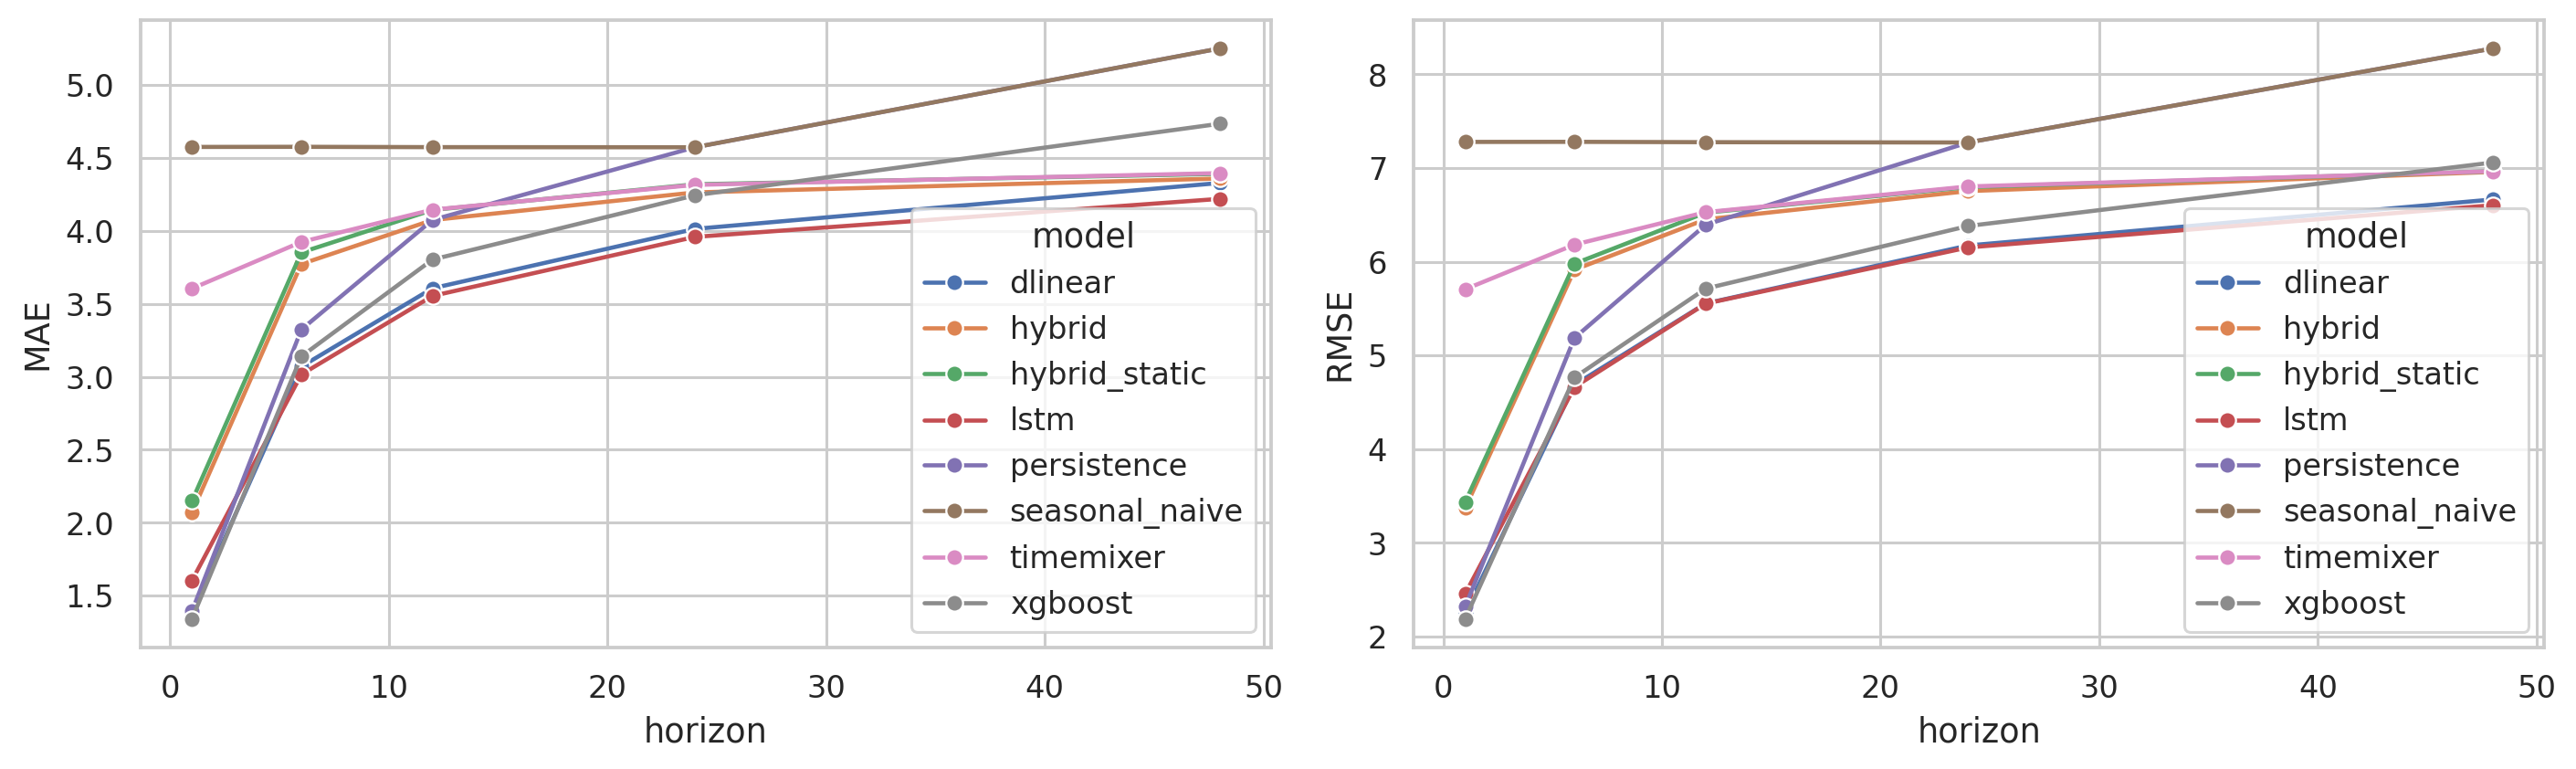
\includegraphics[width=\textwidth]{04_model_metrics.png}
\caption{Locked-test MAE and RMSE by horizon. Final claims must use the completed five-seed multi-station tables rather than a single run.}
\label{fig:model-metrics}
\end{figure*}}{}

The earlier ungated multi-station diagnostic found that rolling calibration
reduced the damage caused by static residual over-correction but did not beat
the strongest matched comparator. That diagnostic motivated the
calibration-gated revision and is archived separately rather than reused as
evidence. The result exporter accepts only complete gated-v2 runs covering all
five stations, seeds 0-4, and the 30-epoch configuration. The hybrid is
called effective only when it improves on the strongest matched comparator
without worsening bias, high-event behavior, or seed stability.

\IfFileExists{generated_results.tex}{% Auto-generated from complete gated-v2 multi-station results.
\begin{table*}[tbp]
\centering
\caption{Locked-test MAE pooled over station--seed runs. Parentheses show dispersion across both stations and seeds; station-specific comparisons are retained in the machine-readable results.}
\label{tab:multistation-mae}
\begin{tabular}{lrrrrr}
\toprule
Model & 1 h & 6 h & 12 h & 24 h & 48 h \\
\midrule
dlinear & 1.390 (0.791) & 3.070 (0.621) & 3.607 (0.558) & 4.014 (0.537) & 4.329 (0.574) \\
hybrid & 2.070 (0.902) & 3.773 (0.519) & 4.075 (0.502) & 4.264 (0.489) & 4.359 (0.472) \\
hybrid\_static & 2.149 (0.906) & 3.853 (0.531) & 4.144 (0.515) & 4.320 (0.494) & 4.391 (0.460) \\
LSTM & 1.604 (0.708) & \textbf{3.016 (0.578)} & \textbf{3.555 (0.541)} & \textbf{3.959 (0.519)} & \textbf{4.220 (0.536)} \\
persistence & 1.394 (0.816) & 3.324 (0.769) & 4.076 (0.748) & 4.574 (0.655) & 5.251 (0.709) \\
seasonal\_naive & 4.576 (0.645) & 4.577 (0.648) & 4.574 (0.650) & 4.574 (0.655) & 5.251 (0.709) \\
timemixer & 3.605 (0.577) & 3.925 (0.540) & 4.146 (0.518) & 4.316 (0.483) & 4.396 (0.469) \\
XGBoost & \textbf{1.341 (0.751)} & 3.140 (0.576) & 3.804 (0.559) & 4.244 (0.540) & 4.735 (0.519) \\
\bottomrule
\end{tabular}
\end{table*}
The hybrid won 0/25 matched comparisons against the strongest non-hybrid comparator, giving a 23.33\% average MAE gap, while still improving compact TimeMixer.

\begin{table}[tbp]
\centering
\caption{Pooled secondary metrics across all stations, horizons, and seeds. Lower is better for MAE, RMSE, and sMAPE; higher is better for \(R^2\).}
\label{tab:secondary-metrics}
\small
\begin{tabular}{lrrrr}
\toprule
Model & MAE & RMSE & sMAPE & \(R^2\) \\
\midrule
LSTM & \textbf{3.271} & 5.086 & 39.374 & \textbf{0.446} \\
dlinear & 3.282 & \textbf{5.066} & \textbf{39.321} & 0.444 \\
XGBoost & 3.453 & 5.222 & 40.526 & 0.404 \\
hybrid & 3.708 & 5.890 & 43.152 & 0.278 \\
persistence & 3.724 & 5.890 & 43.845 & 0.230 \\
hybrid\_static & 3.771 & 5.940 & 44.049 & 0.268 \\
timemixer & 4.078 & 6.437 & 47.304 & 0.178 \\
seasonal\_naive & 4.710 & 7.477 & 53.853 & -0.104 \\
\bottomrule
\end{tabular}
\end{table}
DLinear and LSTM are practically tied in pooled MAE (3.282 versus 3.271); DLinear leads pooled RMSE and sMAPE.

\begin{table}[tbp]
\centering
\caption{Paired block-bootstrap summary for hybrid minus TimeMixer absolute error. Negative values favor the gated hybrid over its TimeMixer base.}
\label{tab:bootstrap-timemixer}
\small
\begin{tabular}{rrrr}
\toprule
Horizon & Mean diff. & 95\% low & 95\% high \\
\midrule
1 & -1.535 & -1.730 & -1.350 \\
6 & -0.152 & -0.209 & -0.095 \\
12 & -0.071 & -0.120 & -0.023 \\
24 & -0.052 & -0.111 & 0.008 \\
48 & -0.037 & -0.100 & 0.027 \\
\bottomrule
\end{tabular}
\end{table}
Bootstrap evidence supports only the narrower claim that gating helps compact TimeMixer.

\begin{table}[tbp]
\centering
\caption{Common-history sensitivity for the hybrid model. Values are MAE changes after restricting every station to a 2021-start training history; negative values favor the common-history run.}
\label{tab:history-sensitivity}
\begin{tabular}{lrrrr}
\toprule
Grouping & Mean $\Delta$MAE & Median $\Delta$MAE & Improved & Worsened \\
\midrule
All station--horizon cells & 0.012 & 0.019 & 8 & 17 \\
1 h horizons & 0.042 & 0.003 & 1 & 4 \\
6 h horizons & 0.112 & 0.102 & 1 & 4 \\
12 h horizons & 0.014 & 0.042 & 1 & 4 \\
24 h horizons & -0.026 & 0.019 & 2 & 3 \\
48 h horizons & -0.083 & 0.011 & 3 & 2 \\
\bottomrule
\end{tabular}
\end{table}
}{}

Relative to its intended TimeMixer base, the gated rolling hybrid reduced
pooled MAE at every horizon: by 42.58\% at 1 hour, 3.86\% at 6 hours,
1.72\% at 12 hours, 1.20\% at 24 hours, and 0.84\% at 48 hours. Thus the
residual stage was effective as a correction to TimeMixer, especially at the
shortest horizon, even though it did not become the strongest model in any of
the 25 station-horizon comparisons. LSTM had the lowest pooled MAE overall
(3.271), while the hybrid achieved 3.708 and TimeMixer achieved 4.078.

\subsection{Forecast behavior beyond average error}
\label{sec:results-high}

Average error can hide peak underprediction. The fixed training-set 90th-percentile threshold is therefore evaluated through event MAE, recall, and false-alarm rate. The 24-hour trace and residual views complement these metrics by exposing smoothing and peak-miss behavior that is not visible from a single aggregate error statistic.

\IfFileExists{../figures/05_forecast_diagnostics.png}{
\begin{figure*}[tbp]
\centering
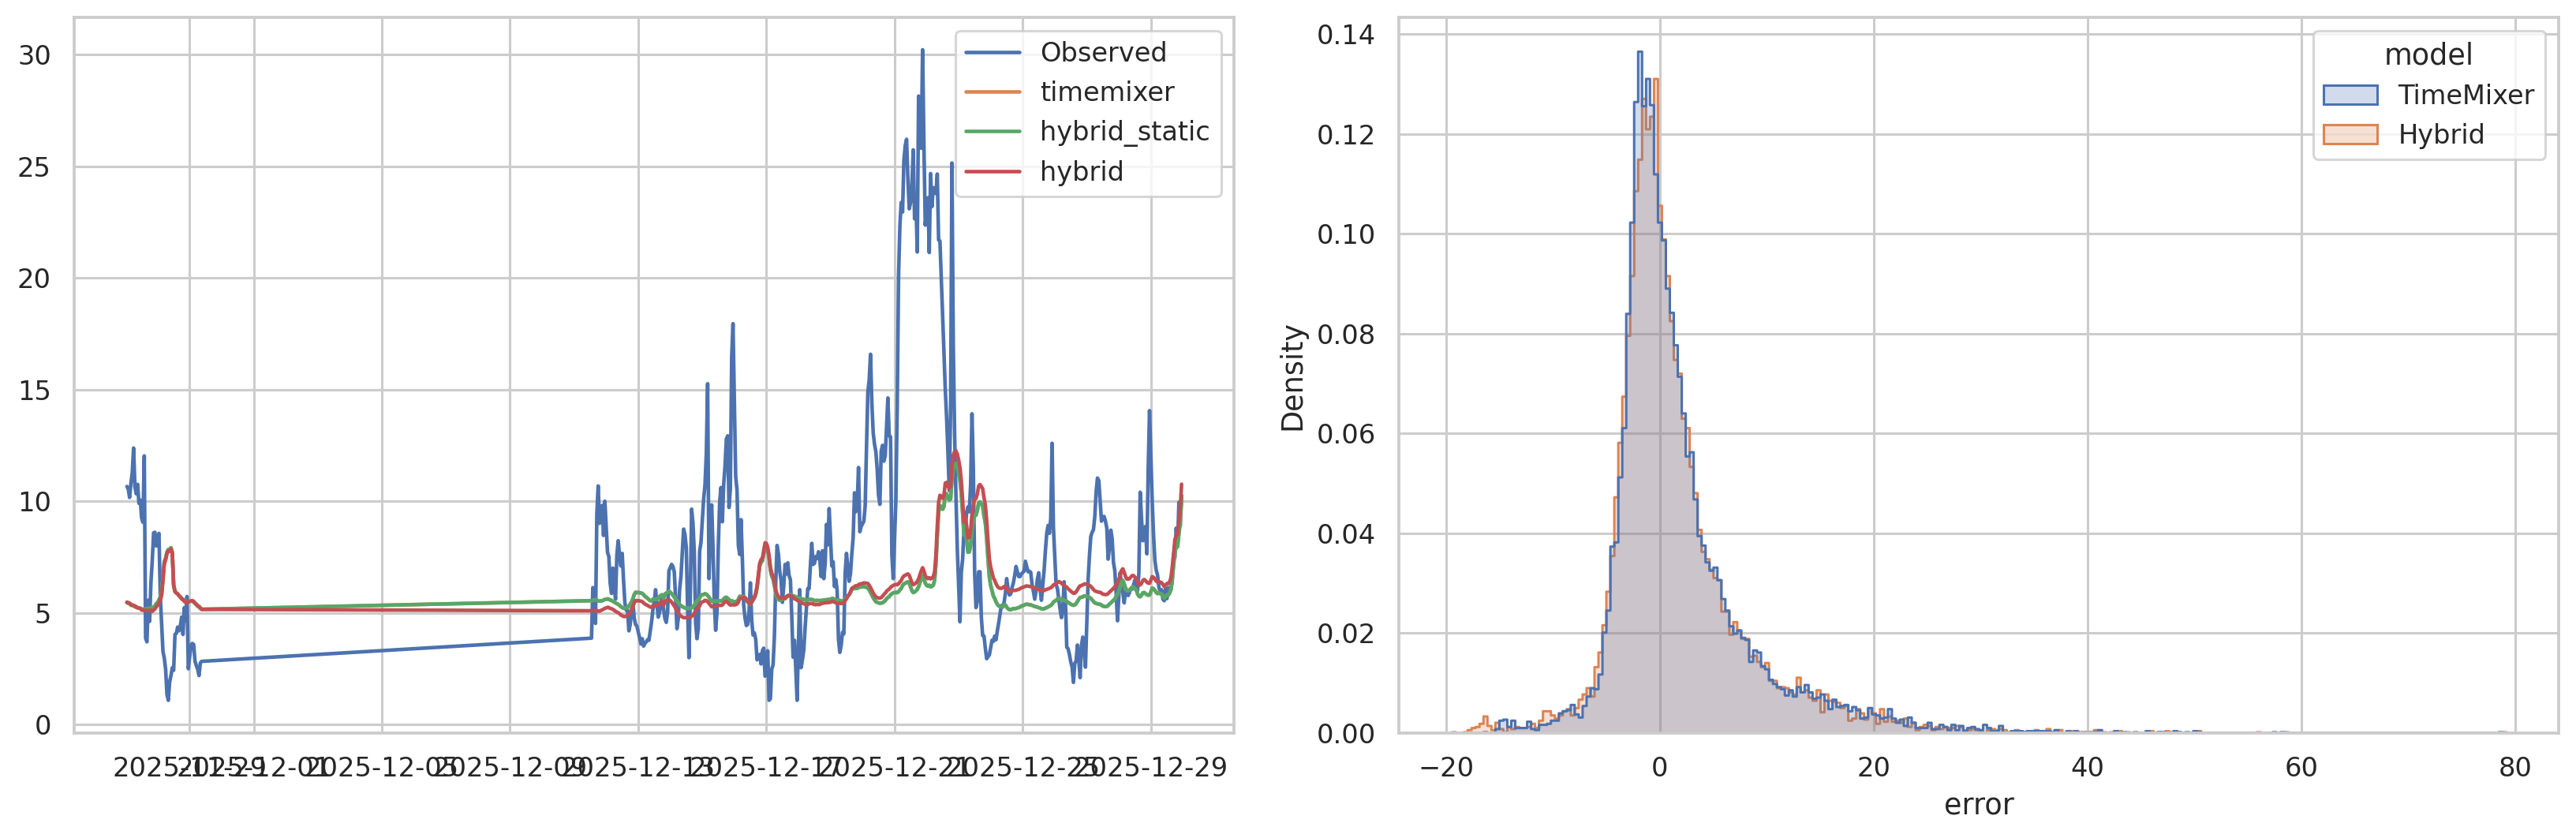
\includegraphics[width=\textwidth]{05_forecast_diagnostics.png}
\caption{Forecast-behavior diagnostics at the 24-hour horizon. The trace and residual views expose smoothing and peak-miss behavior that is not visible from a single average-error statistic.}
\label{fig:forecast-diagnostics}
\end{figure*}}{}

\subsection{What the ablations and SHAP summaries establish}
\label{sec:results-ablation}

The ablation study is intentionally same-origin and chronological. It
distinguishes the TimeMixer base, ungated robust correction,
calibration-gated static correction, rolling correction, and reduced-feature
variants. This allows the paper to separate nonlinear residual fit, protection
against over-correction, and adaptation to recent drift.

The ablation identifies over-correction as the main failure mode of the
ungated residual learner. At horizons 12, 24, and 48 hours, its pooled MAE was
6.020, 6.420, and 6.632, respectively. Calibration gating reduced these values
to 4.144, 4.320, and 4.391, and rolling calibration further reduced them to
4.075, 4.264, and 4.359. The gate selected zero correction in 56.8\% of all
station-seed-horizon fits. Mean gate weight was 0.930 at 1 hour but no more
than 0.158 at longer horizons, showing that strong residual correction was
supported primarily at short lead time.

SHAP summaries describe how the fitted residual booster allocates prediction contribution across base forecasts, embedding coordinates, and origin context. Because embedding dimensions are learned latent coordinates, interpretation is primarily grouped: total base-forecast contribution, total embedding contribution, and named context contribution by horizon. These summaries are predictive diagnostics and must not be interpreted as causal effects of instrument or calendar variables on pollution.

\IfFileExists{../figures/06_residual_ablation.png}{
\begin{figure*}[tbp]
\centering

\includegraphics[width=\textwidth]{06_residual_ablation.png}
\caption{Residual ablation separating the TimeMixer base, ungated robust correction, held-out calibration gating, rolling calibration, and reduced feature variants. SHAP detail is moved to the supplement.}
\label{fig:shap-ablation}
\end{figure*}}{}

\IfFileExists{../figures/07_seed_variability.png}{
\IfFileExists{../figures/08_bootstrap_forest.png}{
\begin{figure*}[!t]
\centering
\begin{minipage}[t]{0.49\textwidth}
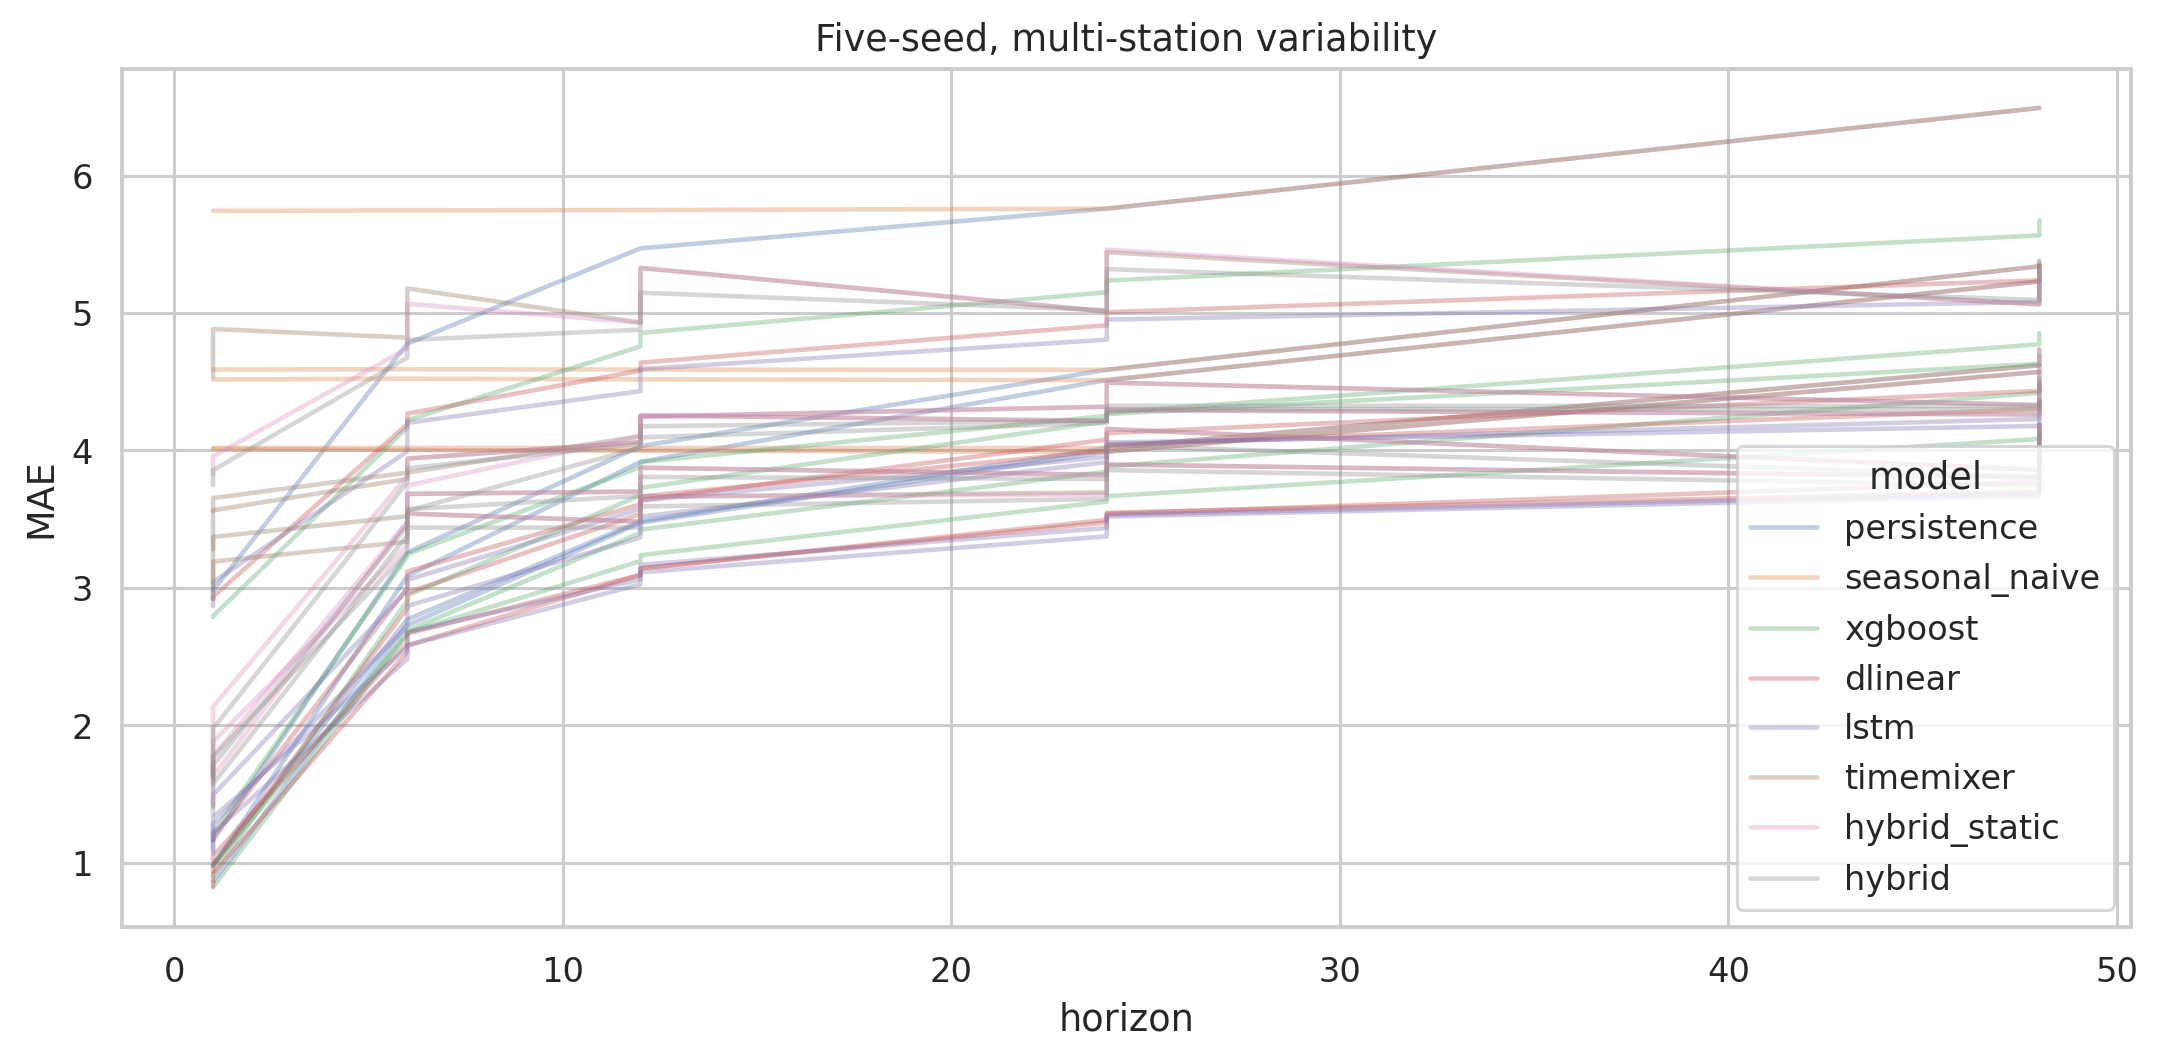
\includegraphics[width=\linewidth]{07_seed_variability.png}
\end{minipage}\hfill
\begin{minipage}[t]{0.49\textwidth}
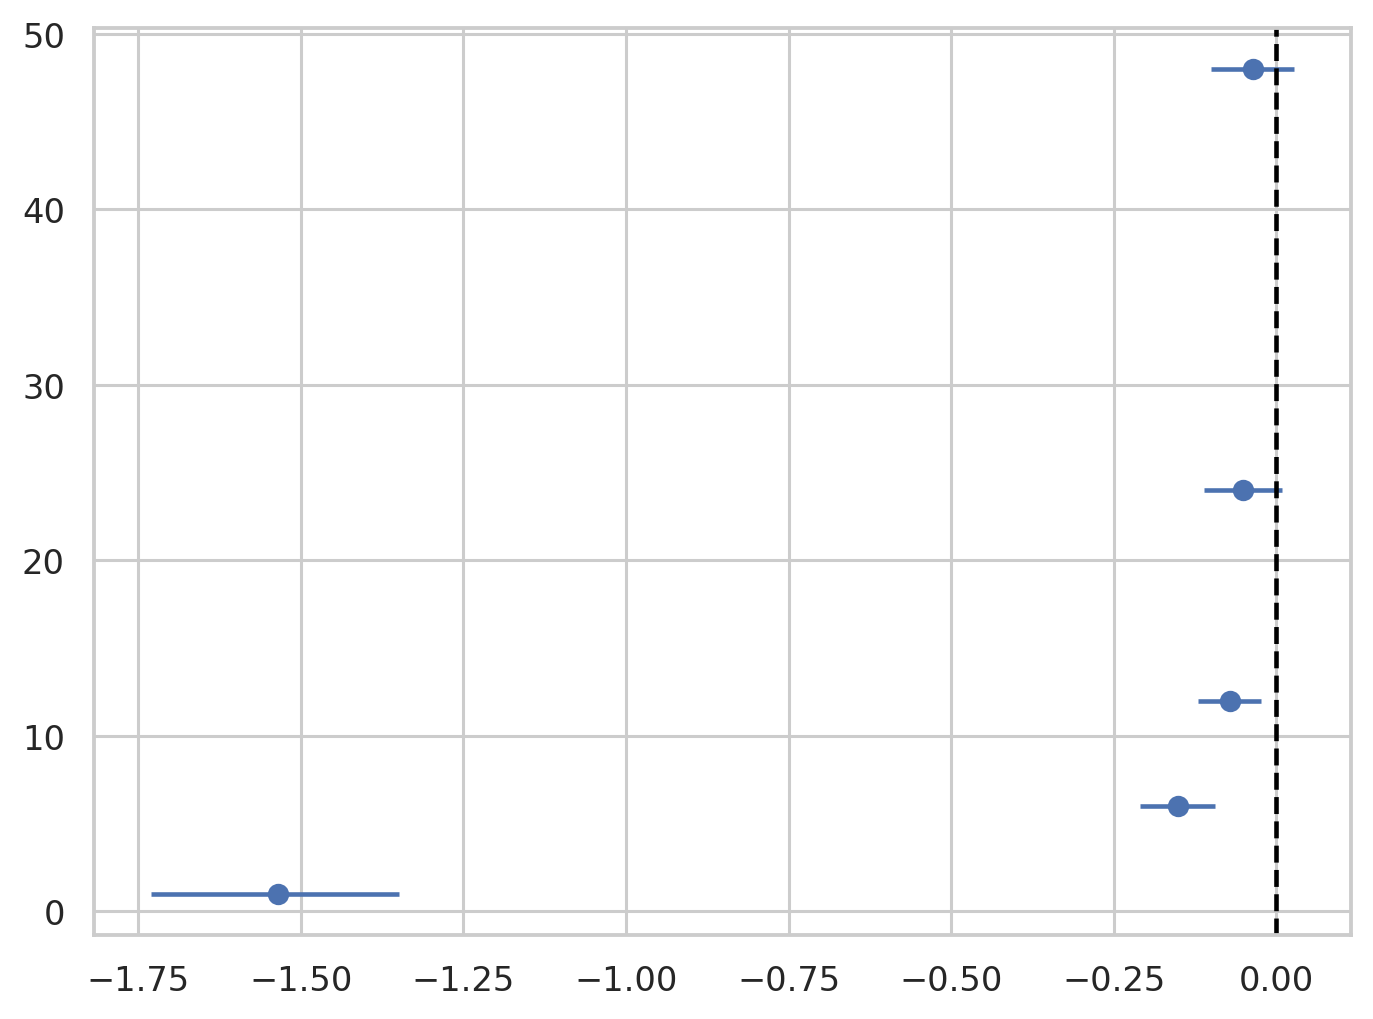
\includegraphics[width=\linewidth]{08_bootstrap_forest.png}
\end{minipage}
\caption{Five-seed variability and paired moving-block bootstrap evidence.}
\label{fig:bootstrap}
\end{figure*}}{}}{}
\FloatBarrier

\subsection{Five-seed experimental setting}
\label{sec:results-seeds}

The confirmatory experiment uses seeds 0-4 and a maximum of 30 epochs with early stopping. Results are reported as mean and standard deviation across seeds, while station-horizon effectiveness is measured against the strongest non-hybrid comparator at the same station and horizon.

\section{Discussion}
\label{sec:discussion}

Across all station--seed--horizon rows, hybrid MAE was 3.708, compared with 4.078 for compact TimeMixer, 3.282 for DLinear, and 3.271 for LSTM. Thus the gate improves the base model but does not make it globally competitive. The gate selected zero correction in 56.8\% of fits, and common-history sensitivity changed hybrid MAE by only \( +0.012 \), so unequal historical depth does not reverse the conclusion.


These findings distinguish two definitions of effectiveness. First, the
gated residual architecture consistently improved its TimeMixer base in
pooled horizon-level MAE, and 81 of 125 station-seed-horizon block-bootstrap
intervals lay entirely below zero for the hybrid-minus-TimeMixer absolute
error difference. Second, it did not outperform the strongest alternative
model selected independently at each station and horizon. The first result
supports the gate as a safeguard and residual-correction mechanism; the
second rejects a broader superiority claim.

The pattern is consistent with lead-time-dependent information content.
At one hour, recent PM2.5 lags are highly predictive and the residual booster
can exploit origin-safe tabular context, so the gate retains most of the
correction. At longer horizons, calibration frequently chooses a zero or
small correction and the hybrid approaches TimeMixer. LSTM and DLinear then
remain stronger because their sequence representations provide a better base
trajectory for this PM2.5-only setting. Adding meteorological forecasts,
regional transport indicators, or a stronger sequence backbone may therefore
be more consequential than increasing residual-booster capacity.

\section{Limitations and Threats to Validity}
\label{sec:limitations}

\paragraph{Internal validity.}
Overlapping sequence windows create serial dependence. Chronological splitting and block-based paired inference reduce but do not eliminate this dependence. Repeated inspection of locked-test results followed by hyperparameter changes would invalidate the confirmatory interpretation. Configuration and prediction files are therefore saved to make changes auditable.

\paragraph{Construct validity.}
Station-level PM2.5 mass concentration is not personal exposure. The training-set 90th percentile is an analytical event threshold rather than a regulatory or health category. Different metrics measure different failure modes: a low MAE can coexist with poor high-event recall, negative bias at peaks, or excessive false alarms.

\paragraph{External validity.}
The experiment covers two urban-traffic, two urban-background, and one rural
UK station, improving on a single-site analysis. It does not establish
generalization to industrial sites, non-UK monitoring networks, or unseen
stations because every station is fitted independently. Leave-one-station-out
transfer and replication under different regulatory monitoring systems remain
necessary.

\paragraph{Data quality and sample selection.}
The conservative missingness policy avoids long fabricated trajectories but
changes the admissible sample toward periods with complete monitoring. HP1's
absent 2016-2018 block, BIR\_A4540's 2021 start, and CHB's reduced 2024
coverage also produce unequal effective sample sizes across stations. Annual
coverage, gap inventories, and rejected-window counts expose these
differences. The pre-specified common-2021 training-history sensitivity runner
is provided, but its result is not included in the present confirmatory
evidence; it must be completed before making a robustness claim about unequal
history length. Neither analysis can remove selection caused by non-random
monitoring outages.

\paragraph{Measurement regime.}
Instrument type can be predictive because measurement response differs or because the replacement coincides with changes in traffic, policy, weather, and emissions. Its SHAP contribution cannot separate these mechanisms. A causal sensor comparison would require collocated parallel measurements or a calibration study.

\paragraph{Omitted physical drivers.}
The PM2.5-only design isolates autoregressive information and simplifies deployment, but it omits meteorology, traffic, co-pollutants, regional transport, and event indicators. Sudden episodes caused by these drivers may be fundamentally difficult to predict from concentration history alone.

\paragraph{Ethics and communication.}
The model is not an official warning system and should not replace monitored observations or public-health guidance. A user-facing deployment should communicate update time, missingness, uncertainty, instrument status, and abstention conditions. False reassurance during high pollution can be more harmful than a conservative warning.

\section{Future Work}
\label{sec:future}

The first extension is \emph{spatial transfer beyond independent
station-level fitting}. The present study repeats a common locked protocol
across urban-traffic, urban-background, and rural stations, but it does not
train on one set of stations and forecast an unseen station. A stronger
external-validity design should therefore add industrial and suburban sites
and evaluate leave-one-station-out transfer.

The second extension is \emph{forecast-available exogenous information}. Meteorology, traffic intensity, co-pollutants, and regional transport indicators may explain episodes that historical PM2.5 alone cannot anticipate. These inputs should be added only under the same origin-availability rule so that forecast-time information and observation-time information are not confused.

The third extension is \emph{adaptive regime handling}. The documented instrument transition is treated here as an observed context variable. Future work could test explicit domain adaptation, change-point detection, or regime-specific calibration while retaining a common locked-test evaluation.

\section{Conclusion}
\label{sec:conclusion}

This paper evaluates a leakage-controlled TimeMixer-XGBoost framework for direct PM2.5 forecasting at five horizons. The workflow begins with an explicit data audit, preserves a 69-day outage and measurement-regime transition, and separates training, neural early stopping, residual calibration, and locked testing. TimeMixer supplies multiscale forecasts and embeddings; horizon-specific XGBoost models attempt to learn the remaining error.

The gated hybrid won 0 of 25 matched comparisons and achieved mean relative improvement of -23.33\%. The best pooled model was LSTM (MAE 3.271). The common-history sensitivity analysis changed hybrid MAE by only \(+0.012\) on average across station--horizon cells, so the unequal-history check does not reverse the main interpretation. The result does not support a superiority or state-of-the-art claim. Claims are therefore restricted to the completed matched protocol and do not imply global SOTA.


\section*{Data and Code Availability}
The project repository contains the supplied raw UK-Air record, preprocessing and modeling source code, tests, notebooks, figure-generation scripts, experiment runners, result schemas, a dashboard, and manuscript source. Users should verify UK-Air licensing conditions and preserve source attribution before redistributing the original data.

\section*{Conflict of Interest}
The author declares no conflict of interest.

\clearpage
\begingroup
\small
\bibliographystyle{unsrt}
\bibliography{refs}
\endgroup

\end{document}
